%!TEX root = ../document.tex
\chapter{Leistungsbewertung} 

	\todo{chap:Grundlagen sec:Precision Recall}

	\todo{chap:Grundlagen sec:Konfidenzen}   

	\section{Messung der Qualität}

		Es werden nun einige Kennzahlen zur Messung der Qualität der Ergebnisse eingeführt.
		Diese werden anhand der untersuchten Hierarchieebene unterteilt.
		Die Städteebene, also die unterste Hierarchieebene, wird dabei anders behandelt als die restlichen Hierarchieebenen.

		Auf der untersten Ebene werden Fehlerdistanzen verwendet.
		Diese geben an wie weit die tatsächliche geografische Position, von der ein Tweet versendet wurde, von der durch die Geolokalisierung zugeordneten geografischen Position (die geografischen Koordinaten der Stadt) entfernt ist.
		Dies lässt eine Detailanalyse der Ergebnisse zu.

		Auf den höheren Ebenen, die eine größere geografische Region beschreiben, ist dies allerdings nicht sinnvoll.
		Ein große geografische Region kann nicht durch einen einzelnen Punkt beschrieben werden. 
		Es wird deshalb nur entschieden ob die Geolokalisierung dem untersuchten Tweet die korrekte geografische Region zuordnet. 
		Einfach ausgedrückt: Ist der Tweet tatsächlich aus der geografischen Region abgesendet worden die ihm durch die Geolokalisierung zugeordnet wurde?
		Es werden also Treffer und Nicht-Treffer gegenübergestellt. 
		
		\subsection{Kennzahlen zur Qualitätsbewertung auf Städteebene}

			Wie bereits erwähnt sollen Fehlerdistanzen verwendet werden. 
			$x^f_{i}$ gibt die geografische Position eines Tweets $i$ an, welche durch die Geolokalisierung bestimmt wurde.
			$x^r_{i}$ gibt die reale geografische Position des Tweets $i$ an. 
			Die Funktion $dist(x,y)$ gibt die Distanz zwischen geografischen Positionen $x$ und $y$ an.

			\subsubsection{Ergebnismenge}

				Unter der Ergebnismenge wird die Anzahl derjenigen Tweets aus den Testdatensätzen verstanden, denen durch die Geolokalisierung eine Georeferenz zugeordnet werden konnte.
				Dabei wird die Korrektheit der zugeordneten Georeferenz nicht berücksichtigt.
				Die Ergebnismenge wird in den Formeln mit $|erg|$

			\subsubsection{Durchschnittliche Fehlerdistanz} 

				Dabei wird die Summe der Fehlerdistanzen durch die Ergebnismenge geteilt.
				Die durchschnittliche Fehlerdistanz $x_{avg}$ errechnet sich durch die Formel:

				\begin{equation}
					x_{avg}=\frac{\sum_{i=0}^{|erg|}{dist(x^f_i,xr_i)}}{|erg|}
				\end{equation}	


			\subsubsection{Quantile der Fehlerdistanzen}

				Ein p-Quantil gibt einen Schwellwert an.
				Das p-Quantil sagt aus, das der p-te Teil einer Menge an Werten unter dem angegeben Wert für das p-Quantil liegt.
				Für einen Wert von 30 für das 0,25-Quantil bedeutet dies, dass 30\% der Werte in der Gesamtmenge unter 30 liegen.

				Um die Quantile zu bestimmen wird zunächst die Liste aller Fehlerdistanzen aufsteigend sortiert.
				Danach kann der Wert durch folgende Formel bestimmt werden. 


			\subsubsection{Median der Fehlerdistanzen}


		\subsection{Kennzahlen zur Qualitätsbewertung Verwaltungseinheiten erster und zweiter Ordnung und Länderebene} 

			\subsubsection{True Positive}

			\subsubsection{False Positive}  

			\subsubsection{Precision}  

			\subsubsection{Recall} 

			\begin{figure}[!ht]
	
						\centering
						\makebox[\textwidth]{
						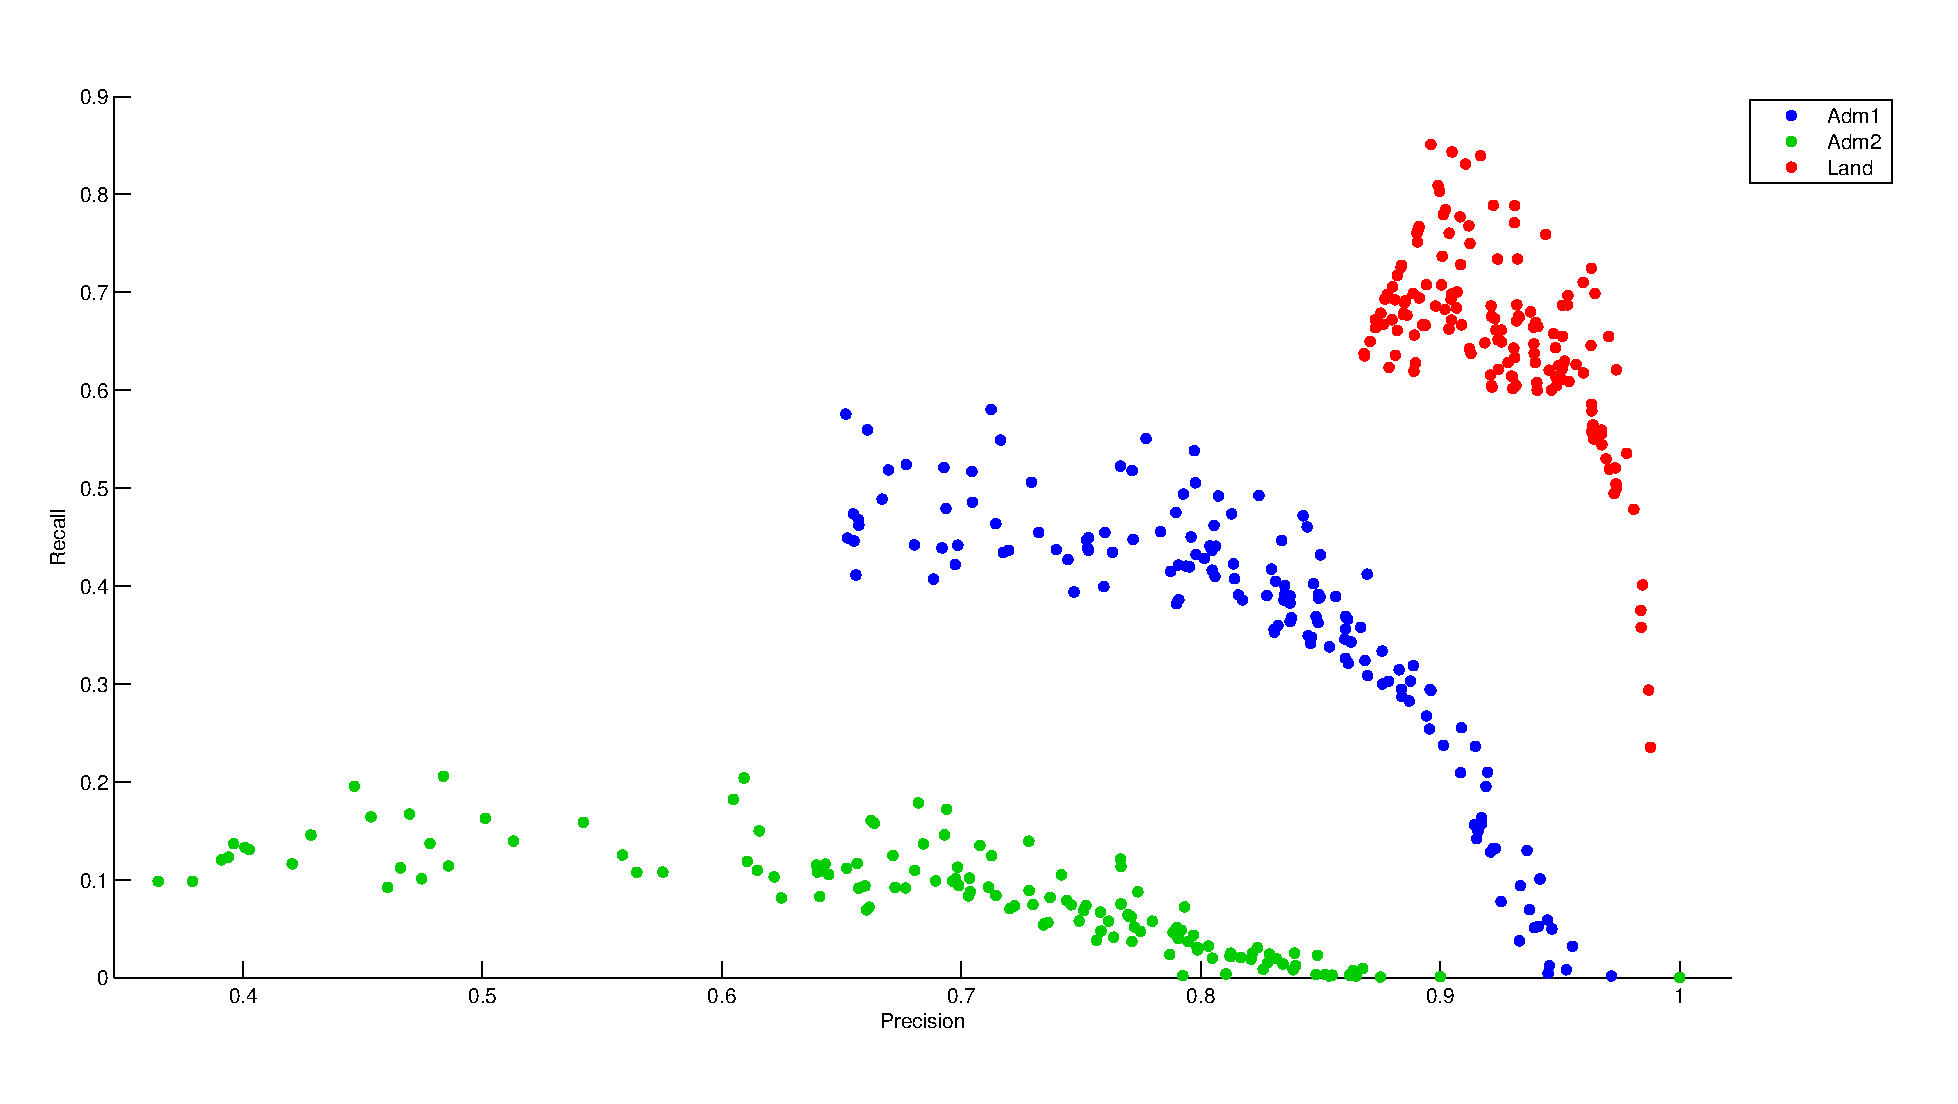
\includegraphics[scale=0.5]{matlabPlot/precRecallAdm1Adm2Cou.eps} 
						} 
						\caption{Precision-Recall Diagramm auf Adm1, Adm2 und Länderebene}
						\label{img:relHaufBsp}
					
				\end{figure}

	\section{Bestimmung Schwellwerte} 
		
		\todo{chap:Lesitungsbewertung sec:Bestimmung Schwellwerte} 
		Ergebnisse Kontrolldaten.
		Angabe Schwellwerte über Random 2D Array. 
		Darstellung in Matlab.
		Maximum finden. 

	\section{Naiver Ansatz}
		
		\todo{chap:Lesitungsbewertung sec:Naiver Ansatz} 
		Im Vergleich zu einem naiven Ansatz.
		Google Maps API V3 ohne Vorverarebitung 
		Precision/Recall. 


	\section{Vergleich zu früheren Ansätzen auf Nutzer-Standort}
		
		\todo{chap:Lesitungsbewertung sec:Vergleich zu früheren Ansätzen auf Nutzer-Standort} 

	\section{Vergleich zu früheren Ansätzen NLP}
		
		\todo{chap:Lesitungsbewertung sec:Vergleich zu früheren Ansätzen NLP}

	\section{Fazit}   

		\todo{chap:Lesitungsbewertung sec:Fazit}


		\subsection{Wahl der Schwellwerte zur Justierung der Genauigkeit und der Trefferquote}

			Die Wahl der beiden Schwellwerte ist abhängig von den Anforderungen.
			Dabei ist die gewünschte geografische Hierarchie der zurückgegeben Georeferenz ein Faktor.
			Und die gewünschte Genauigkeit und Trefferquote.
			
			\paragraph{Gewünschte Hierarchieebene der Georeferenz}

				

			\paragraph{Genauigkeit und Trefferquote} 

				Der zweite Faktor ist die gewünschte Trefferquote und die Genauigkeit.

				Umso niedriger der Schwellwert $s_{rel}$ ist, umso größer wird die Wahrscheinlichkeit Referenzwerte zu wählen die keinen geografischen Bezug haben.
				Daraus resultieren mehr fehlerhafte Zuordnungen einer Georeferenz.
				Wodurch die Genauigkeit schlechter wird.
				Dadurch können allerdings mehr Georeferenzen zugeordnet werden, wordurch die Trefferquote verbessert wird.
				Umso höher der Schwellwert $s_{rel}$ gewählt wird umso mehr Referenzwerte mit geografischem Bezug werden verworfen.
				Die Wahrscheinlichkeit, dass die gewählten Referenzwerte tatsächlich geografischen Bezug haben ist allerdings höher.
				Dadurch können weniger Georeferenzen zugeordnet werden.
				Somit sinkt die Trefferquote.
				Allerdings sind die zugewiesenen Georeferenzen sicherer womit die Genauigkeit steigt.

				Der Schwellwert $s_{abs}$ vermeidet, dass Referenzwerte gewählt werden die eine hohe realtive Häufigkeit aufweisen aber aufgrund ihrer geringen Vorkommen nicht relevant sind.
				Die Auswirkungen der Wahl des Schwellwertes $s_{abs}$ verhalten sich Analog zum Schwellwert $s_{rel}$.

			\paragraph{Fazit}

				Die Wahl der Schwellwerte hängt zum einen von der Hierarchieebene und zum anderen von den Anforderungen an die Genauigkeit und die Trefferquote ab.
				In Bezug auf die geografischen Hierarchieebenen sind lediglich separate Schwellwerte für jede geografischen Hierarchieebenen zu bestimmen, da die relativen und absoluten Häufigkeiten sich insgesamt verändern.
				Bezüglich der Genauigkeit und der Trefferquote ist ein Kompromiss zwischen den beiden Werten einzugehen. 
				Die Verbesserung der Trefferquote geht mit einer Verschlechterung der Genauigkeit einher und umgekehrt.
				Es kann also entweder ein Kompromiss gefunden werden der ein Optimum für beide Werte darstellt. 
				Oder einer der Werte wird optimiert.  

	
				\paragraph{Vergleich der relativen Häufigkeiten zu Uni- Bi- und Trigrammen}

					Jedes Element eines Bi- oder Trigrammes kann potenziell einen geografischen Bezug haben. 
					Umso mehr Elemente ein NGramm beinhaltet umso spezieller kann die Beschreibung des geografischen Objekts sein.
					Deshalb können NGramme mit einem höheren Grad ein Objekt genauer beschreiben als NGramme mit einem niedrigeren Grad.

					Allerdings können NGramme mit einem höheren Grad auch eine schlechtere Beschreibung darstellen. 
					Beispielsweise wenn das zusätzliche Element keinen geografischen Bezug hat.

					Bei NGrammen mit einem Grad größer zwei können also zwei Fälle unterschieden werden.

					\begin{enumerate}
						\item Die Kombination aus den Elementen des NGrammes beschreibt einen Ort genauer
						\item Die Kombination aus den Elementen des NGrammes beschreibt einen Ort nicht genauer
					\end{enumerate}

					\subparagraph{Fall1} 

						Ein Beispiel für den ersten Fall ist der Nutzer-Standort "'york"' mit der Nutzer-Zeitzone "'eastern+time+us+canada"'. 
						Durch die Vorverarbeitung werden folgende potenzielle geografische Indikatoren erzeugt.
						\begin{enumerate}		
							\item york
							\item york \textit{eastern+time+us+canada}
						\end{enumerate}		

						Eine Stadt Namens York existiert sowohl in Grossbritannien als auch in den USA.
						Fragt man nun die beiden Referenzwerte in der Georeferenz-Basis ab erhält man folgende Werte:

							\begin{table}[h]
								\centering
									\caption{"'york"'}
									\label{tab:york}
									\begin{tabular}{|l|l|l|l|}
									\hline
									Referenzwert 				& Stadt  	& abs. Häufigkeit & rel. Häufigkeit in \% \\ \hline \hline
									York          				& York (GB) & 97              & 48,3       \\ \hline
									york eastern+time+us+canada & York (US) & 12              & 63,2        \\ \hline
									\end{tabular}
							\end{table}

							Die realtive Häufigkeit für york in Kombination mit der Zeitzone ist höher. 
							Die Zeitzone gibt zusätzliche Auskunft darüber welches York gemeint ist. 
							Die Kombination ist spezieller, kommt deshalb seltener vor und potenziell eher dort wo sie zutrifft. 
							In diesem Fall in York in den USA. 

							In den meisten Fällen beschreibt einer der beiden Indikatoren eine größere geografische Region wie beispielsweise einen Bundesstaat der USA.
							Wird ein weiterer Wert, beispielsweise ein Städtename hinzugenommen, wird die Angabe des Ortes genauer. 
							Die Wahrscheinlichkeit, dass diese Kombination ausserhalb des Ortes auftritt wird geringer. 

					\subparagraph{Fall 2}

						Hier können wiederum 2 Fälle unterschieden werden.

						\begin{enumerate}
							\item Beide Elemente beziehen sich auf unterschiedliche geografische Objekte
							\item Nur ein Element hat geografischen Bezug das andere nicht 
						\end{enumerate}

						Wenn zu einem Referenzwert mit geografischem Bezug ein Element hinzugefügt wird, welches keinen geografischen Bezug hat, beschreibt dies den Ort nicht genauer.
						Es ist zu erwarten, dass die Kombination der Elemente sehr selten vorkommt oder sehr verteilt ist. 
						Ist die Kombination verteilter, so ist der relative Wert geringer als der des einzelnen Referenzwertes mit geografischem Bezug.
						Ist die Kombination seltener kann der Referenzwert bereits durch den Schwellwert $s_{abs}$ aussortiert werden.		

						Wenn zu einem Referenzwert mit geografischem Bezug ein Element hinzugefügt wird, welches zwar geografischen Bezug hat, aber dieses sich auf ein anderes geografisches Objekt bezieht ist dasselbe Verhalten zu erwarten.




\paragraph{Genauigkeit und Trefferquote} 

				Der zweite Faktor ist die gewünschte Trefferquote und die Genauigkeit.

				Umso niedriger der Schwellwert $s_{rel}$ ist, umso größer wird die Wahrscheinlichkeit Referenzwerte zu wählen die keinen geografischen Bezug haben.
				Daraus resultieren mehr fehlerhafte Zuordnungen einer Georeferenz.
				Wodurch die Genauigkeit schlechter wird.
				Dadurch können allerdings mehr Georeferenzen zugeordnet werden, wordurch die Trefferquote verbessert wird.
				Umso höher der Schwellwert $s_{rel}$ gewählt wird umso mehr Referenzwerte mit geografischem Bezug werden verworfen.
				Die Wahrscheinlichkeit, dass die gewählten Referenzwerte tatsächlich geografischen Bezug haben ist allerdings höher.
				Dadurch können weniger Georeferenzen zugeordnet werden.
				Somit sinkt die Trefferquote.
				Allerdings sind die zugewiesenen Georeferenzen sicherer womit die Genauigkeit steigt.

				Der Schwellwert $s_{abs}$ vermeidet, dass Referenzwerte gewählt werden die eine hohe realtive Häufigkeit aufweisen aber aufgrund ihrer geringen Vorkommen nicht relevant sind.
				Die Auswirkungen der Wahl des Schwellwertes $s_{abs}$ verhalten sich Analog zum Schwellwert $s_{rel}$.

			\paragraph{Fazit}

				Die Wahl der Schwellwerte hängt zum einen von der Hierarchieebene und zum anderen von den Anforderungen an die Genauigkeit und die Trefferquote ab.
				In Bezug auf die geografischen Hierarchieebenen sind lediglich separate Schwellwerte für jede geografischen Hierarchieebenen zu bestimmen, da die relativen und absoluten Häufigkeiten sich insgesamt verändern.
				Bezüglich der Genauigkeit und der Trefferquote ist ein Kompromiss zwischen den beiden Werten einzugehen. 
				Die Verbesserung der Trefferquote geht mit einer Verschlechterung der Genauigkeit einher und umgekehrt.
				Es kann also entweder ein Kompromiss gefunden werden der ein Optimum für beide Werte darstellt. 
				Oder einer der Werte wird optimiert.  

	
				\paragraph{Vergleich der relativen Häufigkeiten zu Uni- Bi- und Trigrammen}

					Jedes Element eines Bi- oder Trigrammes kann potenziell einen geografischen Bezug haben. 
					Umso mehr Elemente ein NGramm beinhaltet umso spezieller kann die Beschreibung des geografischen Objekts sein.
					Deshalb können NGramme mit einem höheren Grad ein Objekt genauer beschreiben als NGramme mit einem niedrigeren Grad.

					Allerdings können NGramme mit einem höheren Grad auch eine schlechtere Beschreibung darstellen. 
					Beispielsweise wenn das zusätzliche Element keinen geografischen Bezug hat.

					Bei NGrammen mit einem Grad größer zwei können also zwei Fälle unterschieden werden.

					\begin{enumerate}
						\item Die Kombination aus den Elementen des NGrammes beschreibt einen Ort genauer
						\item Die Kombination aus den Elementen des NGrammes beschreibt einen Ort nicht genauer
					\end{enumerate}

					\subparagraph{Fall1} 

						Ein Beispiel für den ersten Fall ist der Nutzer-Standort "'york"' mit der Nutzer-Zeitzone "'eastern+time+us+canada"'. 
						Durch die Vorverarbeitung werden folgende potenzielle geografische Indikatoren erzeugt.
						\begin{enumerate}		
							\item york
							\item york \textit{eastern+time+us+canada}
						\end{enumerate}		

						Eine Stadt Namens York existiert sowohl in Grossbritannien als auch in den USA.
						Fragt man nun die beiden Referenzwerte in der Georeferenz-Basis ab erhält man folgende Werte:

							\begin{table}[h]
								\centering
									\caption{"'york"'}
									\label{tab:york}
									\begin{tabular}{|l|l|l|l|}
									\hline
									Referenzwert 				& Stadt  	& abs. Häufigkeit & rel. Häufigkeit in \% \\ \hline \hline
									York          				& York (GB) & 97              & 48,3       \\ \hline
									york eastern+time+us+canada & York (US) & 12              & 63,2        \\ \hline
									\end{tabular}
							\end{table}

							Die realtive Häufigkeit für york in Kombination mit der Zeitzone ist höher. 
							Die Zeitzone gibt zusätzliche Auskunft darüber welches York gemeint ist. 
							Die Kombination ist spezieller, kommt deshalb seltener vor und potenziell eher dort wo sie zutrifft. 
							In diesem Fall in York in den USA. 

							In den meisten Fällen beschreibt einer der beiden Indikatoren eine größere geografische Region wie beispielsweise einen Bundesstaat der USA.
							Wird ein weiterer Wert, beispielsweise ein Städtename hinzugenommen, wird die Angabe des Ortes genauer. 
							Die Wahrscheinlichkeit, dass diese Kombination ausserhalb des Ortes auftritt wird geringer. 

					\subparagraph{Fall 2}

						Hier können wiederum 2 Fälle unterschieden werden.

						\begin{enumerate}
							\item Beide Elemente beziehen sich auf unterschiedliche geografische Objekte
							\item Nur ein Element hat geografischen Bezug das andere nicht 
						\end{enumerate}

						Wenn zu einem Referenzwert mit geografischem Bezug ein Element hinzugefügt wird, welches keinen geografischen Bezug hat, beschreibt dies den Ort nicht genauer.
						Es ist zu erwarten, dass die Kombination der Elemente sehr selten vorkommt oder sehr verteilt ist. 
						Ist die Kombination verteilter, so ist der relative Wert geringer als der des einzelnen Referenzwertes mit geografischem Bezug.
						Ist die Kombination seltener kann der Referenzwert bereits durch den Schwellwert $s_{abs}$ aussortiert werden.		

						Wenn zu einem Referenzwert mit geografischem Bezug ein Element hinzugefügt wird, welches zwar geografischen Bezug hat, aber dieses sich auf ein anderes geografisches Objekt bezieht ist dasselbe Verhalten zu erwarten.



	\begin{figure}[!ht]
	
						\centering
						\makebox[\textwidth]{
						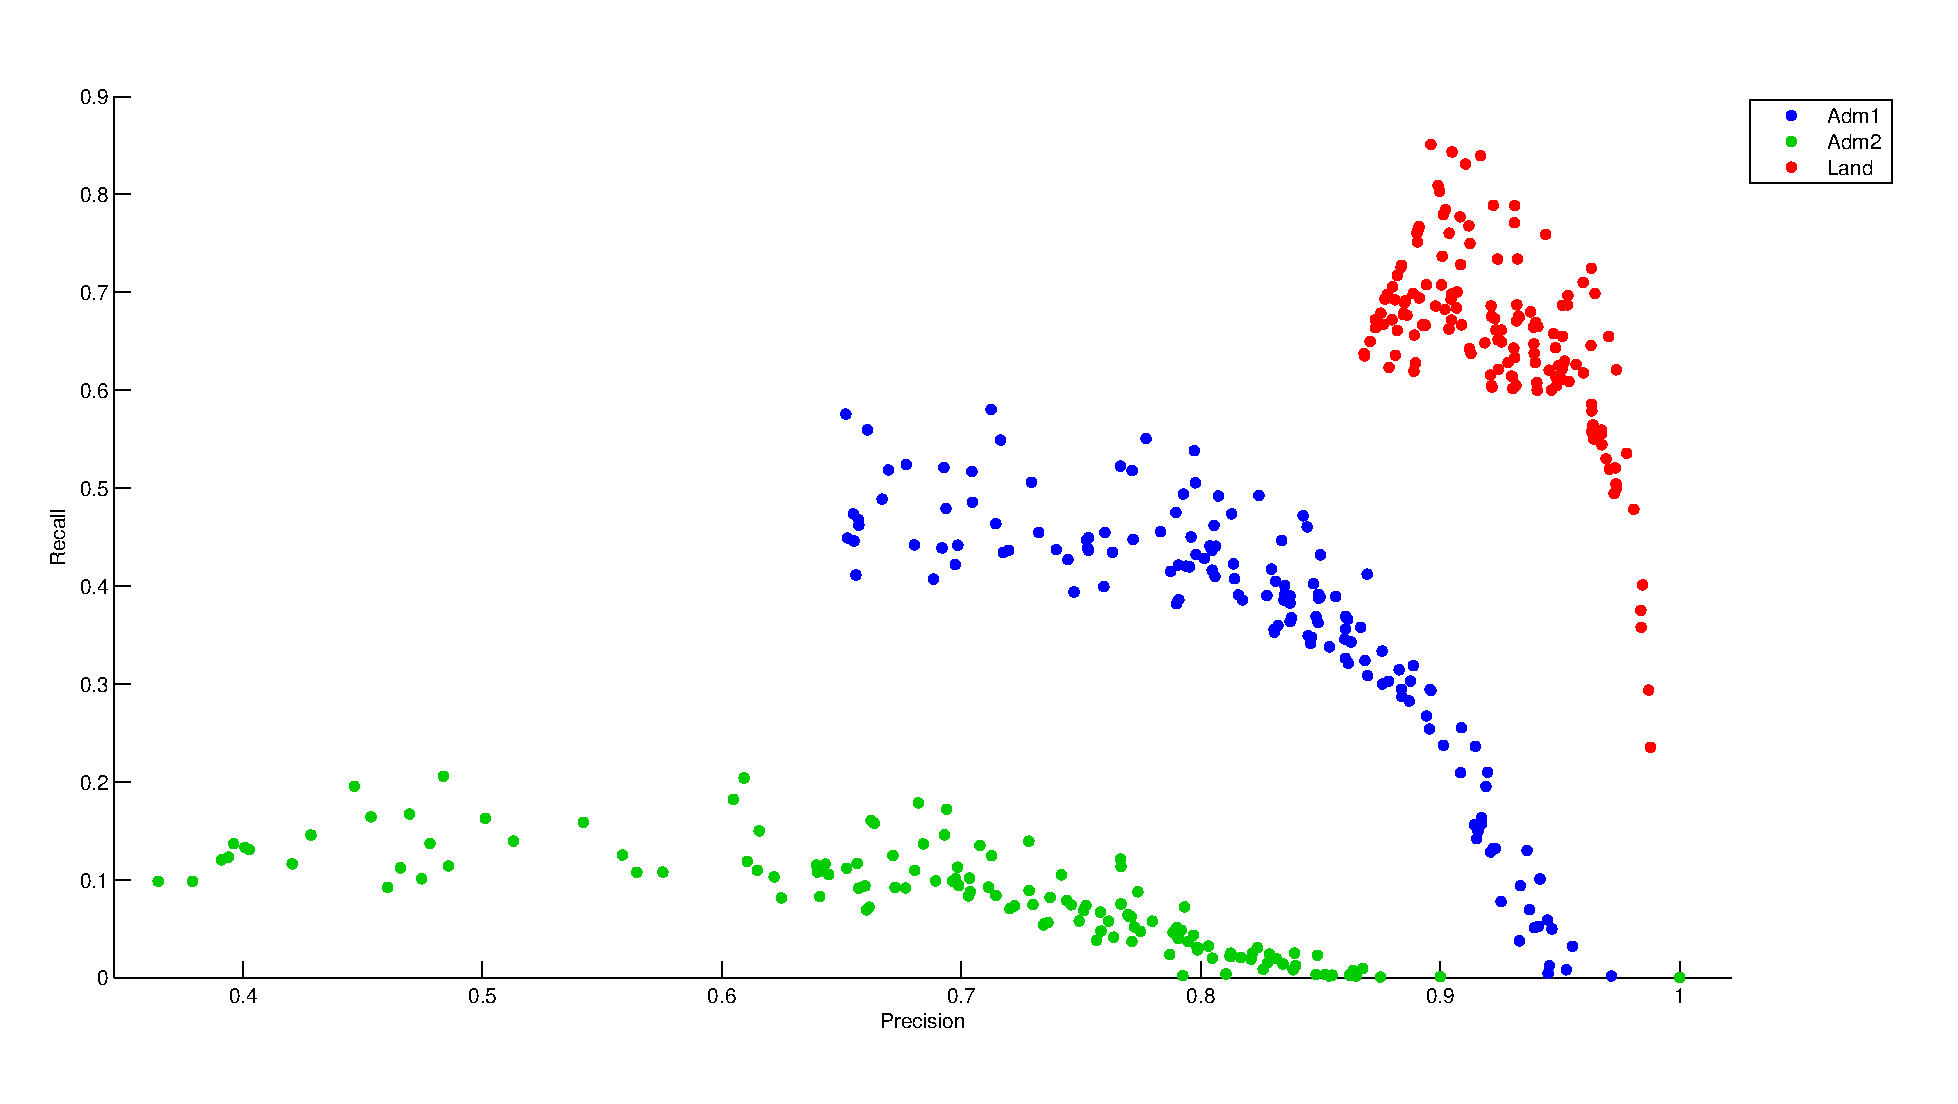
\includegraphics[scale=0.5]{matlabPlot/precRecallAdm1Adm2Cou.eps} 
						} 
						\caption{Precision-Recall Diagramm auf Adm1, Adm2 und Länderebene}
						\label{img:relHaufBsp}
					
				\end{figure}




				\subsection{Ergebnisse Städte}

			In Tabelle \ref{tab:bestErgebnisse} sind die besten Ergebnisse für die einzelnen Kennzahlen dargestellt.
			Die beste Ergebnismenge liegt bei 15819 Tweets (Anteil an Gesamtanzahl der untersuchten Tweets: 79\%) denen eine Georeferenz zugeordnet wurde. 
			Von diesen 15819 Tweets wurden 50\% im Umkreis von 20,43 Kilometern um die ermittelte Georeferenz abgesetzt.

			Die durchschnittliche Fehlerdistanz liegt dabei bei 1423km. 
			Des weiteren wurden die besten erreichten Werte für den Median und die durchschnittliche Fehlerdistanz betrachtet.
			Diese leigen bei 3,24 km für den Median und bei 5,50 km für die durchschnittliche Fehlerdistanz.
			Die Ergebnismenge von 0,08\% und 0,99\% ist sehr gering, es kann sich dabei um Ausreisser handeln.
			Dies macht eine Interpretation der verwendeten Schwellwerte in Bezug auf die Ergebnisse für den Median und die durchschnittlichen Fehlerdistanzen schwierig. 
			Es werden deshalb in Tabelle \ref{tab:bestErgebnisse2000} die besten erzielten Ergebnisse für eine Ergebnissmenge über 2000 ausgewertet.
			Die besten Ergebnisse wurden für dieselben Schwellwerte gemessen. 
			Diese liegen bei 11,15 km für den Median und 253,37 km für die durchschnittliche Fehlerdistanz.
			Es fällt auf, dass sich der Schwellwert für die absolute Häufigkeit gegenüber den besten Ergebnissen für den Median 

			

			\begin{table}[h]
			\centering
			\footnotesize
			\begin{tabular}{|r|r|r|r|r|r|r|}
			\hline
			\multicolumn{1}{|c|}{\begin{tabular}[c]{@{}c@{}}Schwellwert \\ relative \\ Häufigkeit\\ (\%)\end{tabular}} & \multicolumn{1}{c|}{\begin{tabular}[c]{@{}c@{}}Schwellwert\\ absolute \\ Häufigkeit\end{tabular}} & \multicolumn{1}{c|}{\begin{tabular}[c]{@{}c@{}}Ergebnismenge \\(Anteil)\end{tabular}} & \multicolumn{1}{c|}{\begin{tabular}[c]{@{}c@{}}Median\\ (km)\end{tabular}}  & \multicolumn{1}{c|}{\begin{tabular}[c]{@{}c@{}}Durchschn. \\ Fehlerdistanz\\ (km)\end{tabular}} \\ \hline
			2.59                                                                                                       & 6                                                                                                 & \textbf{15819 (79\%)}                                                                                                                           & 20.43                                                                                                                                                & 1423.69                                                                                         \\ \hline
			97.48                                                                                                      & 7                                                                                                 & 198 (0.99\%)                                                                                                                                                    & \textbf{3.24}                                                                                                                                          & 188.57                                                                                          \\ \hline
			91.37                                                                                                      & 101                                                                                               & 16  (0.08\%)                                                                                                                                                 & 6.02                                                                                                                                                     & \textbf{5.50}                                                                                   \\ \hline
			\end{tabular}
			\caption{Beste Ergebnisse}
			\label{tab:bestErgebnisse}
			\end{table}

			\begin{table}[h]
			\centering
			\footnotesize
			\begin{tabular}{|r|r|r|r|r|r|r|}
			\hline
			\multicolumn{1}{|c|}{\begin{tabular}[c]{@{}c@{}}Schwellwert \\ relative \\ Häufigkeit\\ (\%)\end{tabular}} & \multicolumn{1}{c|}{\begin{tabular}[c]{@{}c@{}}Schwellwert\\ absolute \\ Häufigkeit\end{tabular}} & \multicolumn{1}{c|}{\begin{tabular}[c]{@{}c@{}}Ergebnismenge \\(Anteil)\end{tabular}} & \multicolumn{1}{c|}{\begin{tabular}[c]{@{}c@{}}Median\\ (km)\end{tabular}}  & \multicolumn{1}{c|}{\begin{tabular}[c]{@{}c@{}}Durchschn. \\ Fehlerdistanz\\ (km)\end{tabular}} \\ \hline
			65.13                                                                                                      & 10                                                                                                & 2302 (11.51\%)                              & \textbf{11.15}                                                                                                                                                                                                                                                              & \textbf{253.37}                                                                                 \\ \hline
			11.70	& 16 &	10299 (51.50\%)	 &	12.50 &	764.022\\ \hline
			\end{tabular}
			\caption{Weitere Ergebnisse}
			\label{tab:bestErgebnisse2000}
			\end{table}



\cite{Hale2012} nutzen die Yahoo und die Google Geocoding Api um das Userlocation-Feld eingehender zu untersuchen.  


		Durch die Kategorisierung wird deutlich, dass auf dem Nutzer-Standort in Kombination mit der Zeitzone bisher keine NLP ausgeführt wurde. 
		Es ist sinnvoll NLP auf den vorgenannten feldern auszuführen, da die Inhalte ähnlich dynamisch sein können wie im Text Feld.
		Der Nutzer-Standort bietet den Vorteil, dass die Intention ist, dass ein Toponym eingegeben. 

		Es wird selten eine geografische Hierarchie zum abbilden der Positionen verwendet.


	\section{Bewertung}


			\cite{Hecht2011} nimmt eine Detailanalyse des Nutzer-Standortes vor, verwendet diesen allerdings nicht direkt für sein Verfahren zur Geolokalisierung.   


		An die Geolokalsierung werden dabei gewisse Mindestanforderungen bezüglich der Qualität gestellt.
		In der Literatur werden allerdings unterschiedliche Kennzahlen zur Bewertung der Qualität herangezogen.
		Gängige Kennzahlen sind auf Fehlerdistanzen basierende Werte wie die durchschnittliche Fehlerdistanz und der Median der Fehlerdistanzen.
		Aber auch Kennzahlen wie die mittlere quadratische Abweichung der Fehlerdistanzen oder Precision und Recall finden Verwendung. 

		Die Ansätze allein auf Basis der erzielten Ergebnisse zu bewerten würde diesen nicht gerecht werden.

	\section{GAZZETEER UND NACHTEILE}

		Bei einer Abfrage des Toponyms "'Hamburg"' auf ein Ortsverzeichnis, wie geonames.org, würden somit mindestens 31 Georeferenzen als Ergebnis erscheinen.
		Tatsächlich liefert geonames.org folgendes Ergebnis:

		\begin{table}[htpb]
			\caption{Abfrage an geonames.org für Hamburg} 
			\centering
			\begin{tabular}{|c|c|}
				\hline
				Land & Anzahl\\
				\hline\hline
				USA & 29 \\
				\hline
				Süd Afrika & 2 \\
				\hline
				Deutschland & 1 \\
				\hline
				Kanada & 1 \\
				\hline
				Surinam & 1 \\
				\hline
			\end{tabular}
			\label{tab:usCitiesGermanNamesx} 
		\end{table} 

		Dies basiert auf Mehrdeutigkeiten aus dem Ergebnis muss eine Auswahl getroffen werden ohne zusätzliches Wissen über den Ort zu haben getroffen werden.


		Tatsächlich beinhaltet die geonames.org Datenbank keinen dieser Bei- und Spitznamen.
		Durch eine Abfrage an dieses Ortsverzeichnis könnte somit keine Georeferenz bestimmt werden.
		Eine Abfrage in Google Maps hingegen bietet bei Eingabe der oben genannten Bei- und Spitznamen Detroit als Vorschlag an. \footnote{http://de.wikipedia.org/wiki/Detroit (abgerufen Juli 2014)} 


		\textit{Probleme früherer Ansätze auf Gazetteer Basis, es wird für ein Land kein Polygon zurückgegeben sondern ein konkreter Punkt. 
		Messung der Genauigkeit bei Evaluierung auf Länderebene nicht möglich.  
		Ich kann das tun da ich alle test tweets auf eine Stadt abbilde, somit zusätzliche Information über Stadt, Adm1 usw bekomme und somit evaluieren kann ob sich ein Tweet in einem Land befindet, denn auch die ergebnisse haben implizit auch alle anderen geografischen Hierarchieebenen.
		}








	\section{Untersuchungen der Paper}

		Accuracy (Acc). The percentage of correctly predicted locations over all test queries. 
	
